\documentclass[10pt, conference, compsocconf]{IEEEtran}

%Compactitem
\usepackage{paralist}

% Graphics
\usepackage[pdftex]{graphicx}
%\usepackage[tight,footnotesize]{subfigure}
\usepackage{subfigure}

%Table background
\usepackage[table,xcdraw]{xcolor}
% *** GRAPHICS RELATED PACKAGES ***

%degree com
\usepackage{gensymb}





% correct bad hyphenation here
\hyphenation{op-tical net-works semi-conduc-tor}


\begin{document}
%
% paper title
% can use linebreaks \\ within to get better formatting as desired
\title{A Game-Based Approach to Monitor Parkinson's Disease: The bradykinesia symptom classification}


\author{\IEEEauthorblockN{Leonardo Medeiros\IEEEauthorrefmark{1}\IEEEauthorrefmark{2},
Hyggo Almeida\IEEEauthorrefmark{1},
Leandro Dias\IEEEauthorrefmark{3}, 
Mirko Perkusich\IEEEauthorrefmark{1} and
Robert Fischer\IEEEauthorrefmark{2}}
\IEEEauthorblockA{\IEEEauthorrefmark{1}Federal University of Campina Grande, Campina Grande, Brazil}
\IEEEauthorblockA{\IEEEauthorrefmark{2}Federal Institute of Alagoas, Maceio, Brazil}
\IEEEauthorblockA{\IEEEauthorrefmark{3} Federal University of Alagoas, Maceio, Brazil}
}

\maketitle


\begin{abstract}
Parkinson's disease (PD) is a degenerative neurological disorder. It causes motor symptoms such as resting tremor, bradykinesia and gait disorders. The disease's progressive nature requires continuous monitoring of the motor symptoms to assist the neurologist in managing medication. With this purpose, Health Monitoring Systems (HMS) are used as a decentralized healthcare approach. On the other hand, most patients reject the current HMS solutions because they are invasive and stigmatizing. In this work, we present a non-invasive HMS for PD motor symptoms based on games. Because of the nature of games, the approach is able to collect data from patients without reminding them that they are under a disease's treatment. We validated our approach with 30 research subjects divided between PD group and Control group. We used Support Vector Machine (SVM) to identify the occurrence of PD's bradykinesia motor symptoms and reached a classification \textit{precision} of 92.31\%. Furthermore, 90,00\% of the patients approved our HMS considering it as non-invasive and easily integrated into their routine.
\end{abstract}

\begin{IEEEkeywords}
Health Monitoring System; Parkinson's Disease; Game for Health
\end{IEEEkeywords}


\IEEEpeerreviewmaketitle



\section{Introduction}

The symptoms associated with PD are caused by a degeneration of dopaminergic neurons in the substantia nigra. Common treatment focuses on drugs that activate dopamine receptors. However, the medication's effectiveness decreases over the years requiring higher dosages \cite{national2006parkinson}. Due to the complex combination of symptoms and the drugs' harmful side-effects, the patient's quality of life strongly depends on the accurate level of medication. Usually, neurologists determine this medication level based on patient's clinic visits and information from caregivers. On the other hand, continuous monitoring at the patients' home provides more data regarding the patient's symptoms and improves the medication management mainly in the disease's intermediate stages~\cite{national2006parkinson}.

Health Monitoring Systems (HMS) are designed to support continuous treatment by moving healthcare services from the hospital to the patients' home. The goal is to have healthcare services that are more cost-effective, frequent, and convenient to the patient. They enable proactive and preventive diagnosis, early detection and treatment of different diseases, and patient wellness support~\cite{cbmshms2015}. They should be seamlessly integrated into the patients' daily routine~\cite{alemdar2015}. Many HMS approaches and technologies have been developed to track the motor symptoms of PD and related disorders. Most of them use wearable sensors attached to the patients' body or clothes to quantify motor abilities \cite{cbmsparkglove2015}, analyze of handwriting movements~\cite{cbmshandwriting2015} and bradykinesia (slowness of the movement) \cite{ambulatory2010}. A major challenge for such wearable technologies is the patient's acceptance because they may consider these devices disturbing, stigmatizing, or overly interfering with their privacy \cite{alemdar2015}.

A promising approach to overcome those challenges is using games for health improvement. In the last few years, several approaches have been proposed for rehabilitation for elderly users \cite{brox11} and PD patients \cite{atkinson2010,synnott_wiipd_2012}. 

Atkinson and Narasimhan \cite{atkinson2010} developed a video game using a touch sensor to record the players' movements as they try to reach specific targets. Theoretically, this approach facilitates a better medical diagnosis of PD, but no system trial has yet been reported. Synnott \textit{et al.}~\cite{synnott_wiipd_2012} used a commercial game console to capture PD motor symptoms, more specifically, tremor. In this approach, the player has to perform a series of motor tasks presented in the form of mini-games, while holding a Nintendo Wii Remote Control. A metric analyzer provides objective metrics detailing the user performance and records them in an electronic patient diary. This diary also includes the patient's self-reported medication intake and symptom self-rating. 

However, one major disadvantage of focusing on tremor is its dependence of the user's action state \cite{synnott_wiipd_2012}. PD tremor is a rest tremor \cite{national2006parkinson}, and we observed in our own research that the tremor can be suppressed~(mainly unintentionally) while the user is concentrating on a game, specially if the player's hands are involved. So, in our approach we use Ms-Kinect Version 1.0\footnote{www.microsoft.com/en-us/kinectforwindows/} motion sensor, which have accuracy and robustness for full body analysis~\cite{gabel2012}.

In this work we present a game-based approach to monitor PD motor symptoms. Our approach has been built with two major requirements: first, contactless measurement of patient motor symptoms inside the game environment; second, usage of popular consumer electronic devices as input to have a non-invasive, cost-effective solution for home use. Our main goal is to continuously provide neurologists with data regarding patient motor symptoms, while collecting the data of patients without reminding them that they are under a disease's treatment.

We validated our approach with 30 research subjects divided between PD group and Control group. We used a Support Vector Machine (SVM) to identify the occurrence of PD's bradykinesia motor symptom and reached a classification accuracy of 86.66\%. To assess our requirements, we used a survey and evaluated the collected data using GQM. Our goal was to confirm that PD patients perceive our approach as non-invasive and that it could, realistically, be integrated into their routine. The results were positive with acceptance of 90\% of the research subjects. 

This paper is organized as follows: Section~\ref{sec:proposedsystem} introduces the system requirements for our game-based HMS and present our game-based HMS; Section~\ref{sec:experimentalresults} describes the experimental validation with the research subjects. Finally, conclusions and future work are summarized in Section~\ref{conclusion} along with this work's limitations.


\section{HMS Description}\label{sec:proposedsystem}

The game-based HMS uses a contactless motion sensor. In other words, it does not require the players to hold or wear any object. For PD patients, who have motor symptoms, this is a key requirement to enable them to easily play the games. We measure the same type of movement that is commonly used by neurologists to assess PD motor symptoms: arm abduction and adduction. The game engages and entertains the PD patients while collecting data for their monitoring.

\subsection{Requirement Analysis}

PD's motor symptoms are usually monitored through motion sensors or video cameras  \cite{cbmshandwriting2015}. Those devices are difficult to be seamlessly integrated into the user routine. In this work, we use a video game with a motion sensor game controller to monitor the symptoms. The decision to use the controller was based on a requirement analysis performed with health professionals. 

To elicit the system's requirement, We applied a semi-structured interview, which combines structured and open-ended questions to guide the interview according to the interviewee answers \cite{practical_guide_re2012}. The interviews were audio-recorded and transcribed for later analysis through a qualitative research tool, QDA-Miner Lite version 1.2~\footnote{http://provalisresearch.com/products/qualitative-data-analysis-software/freeware/}.  As a result, we identified the system requirements from healthcare professionals associated to scientific references.

We interviewed two neurologists and two physiotherapists. According to them, monitoring the arms adduction and abduction of PD patients helps assessing the medication management and bradykinesia motor symptom, and could be applied for physiotherapy treatment and drug dosage medication. The respondents suggested focusing on the bradykinesia motor symptom due to its debilitating progress \cite{national2006parkinson,ambulatory2010}. Thus, treatment benefits could be correlated with the increase of amplitude and angular velocities of an arm's adduction and abduction movements (Fig.~\ref{fig:abduction}), which could be applied to quantify the bradykinesia. Arm abduction occurs when the arm is moved upward and laterally away from the body. The arm adduction occurs when the arm is returned to anatomical position. 


\begin{figure}[!htb]
  \centering
  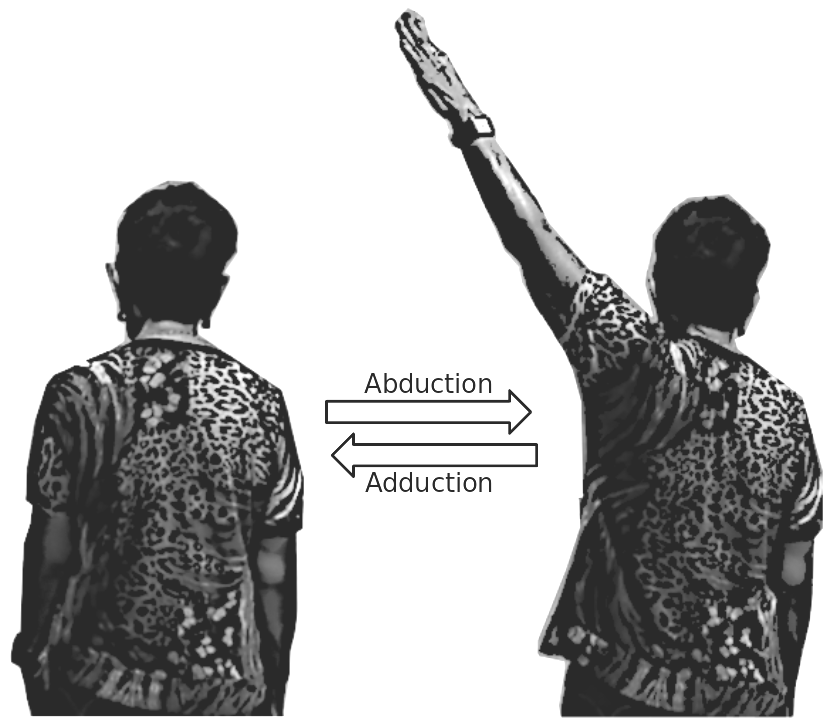
\includegraphics[width=0.4\textwidth]{./img/movaddcutctionartist.png}
  \caption{Movement of abduction and adduction.}
  \label{fig:abduction}
\end{figure}

In summary, we identified the following requirements through literature review and confirmed by the health professionals: 

\begin{compactenum}
    \item Easy and safe to use equipment.
    \item Simple user interface with large fonts and buttons \cite{Uzor:2014:ILU:2611247.2557160}.
    \item Not prompt the players to perform movements that could cause them to suffer physical harm.
    \item Incite the player to perform specific movements that are required for the measurement (i.e., arm abduction and adduction on both sides). The data should allow the system to detect the maximal height and angle of the adduction as well as the speed of the movement.
    \item Contactless measurement.
    \item Measurement in a reasonably short time, because elderly players tire quickly and this affects their motivation and distorts the measurement.
    \item Game with clear and entertaining goal, level of difficulty adapted to the user's skills, user progress display to motivate and distract the players\cite{Uzor:2014:ILU:2611247.2557160}.
    \item Processed data should be presented in a clear and informative visual way to the physician.
    \item Use common consumer electronics such as a game console to reduce cost.
\end{compactenum}

\subsection{System Overview}

 
The system consists of four steps: 1) data acquisition through a video-based full body motion sensor; 2) health game monitor as an acquisition system; 3) signal processing, which includes biomechanical and signal processing patterns identification; 4) and data visualization for the healthcare professional. To provide a measure of the severity of the motor symptoms, the classifier in the signal processing step is trained to distinguish between the moving patterns of healthy subjects, and subjects diagnosed by neurologists as suffering from PD.

Fig.~\ref{img:sysarch} illustrates the client-server architecture of the Health Monitoring System, composed of the Health Game Monitor (HGM) Client, responsible for collecting user data and sending it to the server; and the HGM Server, responsible for processing the data and making the results available to the health professional.

In the HGM Client, the player movements are collected via a MS-Kinect. The device projects a light grid in near infrared onto the player and records it with a video camera to identify and track the 3D coordinates of the player joints and anatomical positions \cite{mcginnis2013biomechanics}. 

The HGM game client was developed using the game engine Unity 3D\footnote{www.unity3d.com} and the Zigfu~\footnote{www.zigfu.com} game component which connects the Ms-Kinnect with the Unity 3D applications. This way, the game was used to capture the player's position and movements in 3D coordinates. The Zigfu and Unity 3D build the core of the HGM client.

By the end of each game session, the user data, including the 3D coordinates of the player's body recorded during the game, are uploaded to the server and saved in the database. From there, the data is processed by a Matlab script\footnote
{http://www.mathworks.com/products/matlab/} to transform coordinates into biomechanical signals and determine the severity or degree of motor symptoms. All technologies involved are under active development, and therefore allow the system to be adapted to (and benefit from) future changes in both hardware and third party software. 

\begin{figure}[!htb]
	\centering
	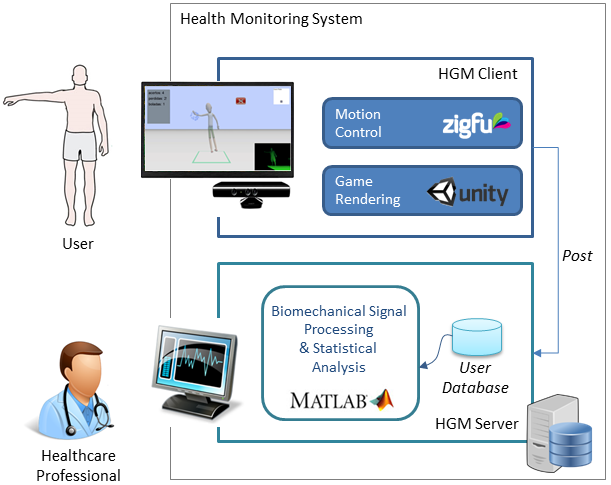
\includegraphics[width=0.475\textwidth]{img/systemarchitecture3.png}
	\caption{System Architecture.}
	\label{img:sysarch}
\end{figure}

Finally, the results are reported to the healthcare professional in a visual and tabular form, featuring direct biomechanical measures that specialists are familiar with from PD diagnosis handbooks \cite{national2006parkinson}, as well as the mechanisms of estimation of the patient's level of motor deficiency \cite{national2006parkinson}.

In the following subsections we detail the two main components of the architecture: the Health Game Monitor client, using the game \textit{Catch the Spheres} as case study; and the HGM server.

\subsection{Health Game Monitor Client: Catch the Spheres}

The Health Monitor Client is the game itself. We have developed a game prototype named \emph{Catch the Spheres} (Fig.~\ref{img:catch}). It is a game in third person in which the players must catch or escape the balls that comes in their direction. There are two types of balls: blue and red. Initially, all the balls are red and some of these suddenly change to blue when approaching the player. The time interval until the ball changes its color may be smaller or larger, depending on the game level selected. The Kinect sensor captures the player movements and replicates them on the character in the center of screen. The player must touch the blue balls with hands and deflect the red balls. The main purpose of the game is to capture the player's movements, when he executes specific actions. The time interval between the moment when the ball changes color and when the ball is captured by the player measures the player's reflexes, while the speed of the movement is calculated from the distance traveled by the 
hands to capture balls.

From the 3D coordinates of the player's body parts acquired by the MS-Kinect motion sensor with position, orientation, velocity and acceleration of the arms and hands, we calculate the angular displacement of adduction and abduction of arm movements \cite{mcginnis2013biomechanics}. As the 3D measurement is noisy, several filtering steps are applied, some in the Kinect system itself. 

During a short game of typically 5 minutes, the player is prompted roughly 10 times to lift their right or left arm to catch a virtual ball approaching from the horizon. The maximal height or angle, the movement's velocity, and the arm to be lifted can thus be indirectly controlled by the trajectory and speed of the ball. A random selection of the trajectories and speeds prevents the player from preparing a movement in advance.

\begin{figure}[!htb]
	\centering
	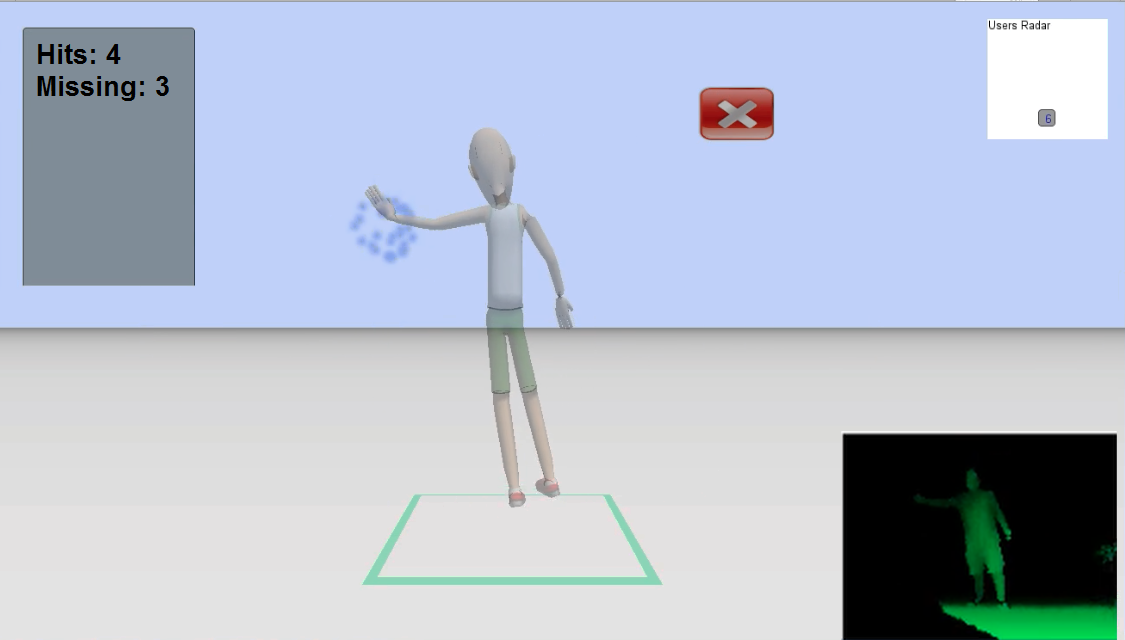
\includegraphics[width=0.475\textwidth]{img/catch_colour.png}
	\caption{Screenshot of the game \emph{Catch the Spheres}. The
		player has just successfully caught a sphere that flew at him from the
		horizon.}
	\label{img:catch}
\end{figure}

\subsection{Health Game Monitor Server: signal processing and statistical analysis}

The data collected through the game is received by the HGM Server at the end of each game session. The complete process for symptom identification can be divided into two phases: biomechanical signal processing and statistical analysis. 

The biomechanical analysis of human movement is part of the diagnosis and treatment process for PD, where the patients are asked to lift their arms, one after the other, at the highest amplitude and velocity they are able to, in order to check the bradykinesia progress. The movement of abduction and adduction are joint actions which involve wrist, shoulder, and hip joints. To identify the movement of adduction and abduction of the arms, it is necessary to use a reference joint. Here, we focus on the wrist joint because its signal has higher amplitude when compared to the other joints. We used the \textit{peaks and valleys} technique to identify the beginning and the end of the movement cycle (Fig.~\ref{fig:signalamplitudepeakvaley}). After the cycle identification, we extract a window length with the cycle movement and transform the MS-Kinect data into angles. Thus, we calculate the angular motion of the movement and consequently the angle displacement of the adduction and abduction movements.

The peak of the amplitude contains the maximum amplitude of each movement. The time spent between the first valley to the peak in each movement cycle is the time taken for the abduction of the arm. The time spent at the peak to the second valley is the time spent for the adduction of the arm. Then, with the maximum amplitude and the time spent in these movements we calculate the angular velocities of abduction and adduction of the arms. However, the acquired signals of the MS-Kinect motion sensors have a lot of noise. In order to remove incomplete movements we designed a data filter which extracts the mean vector and removes outliers. The output of this phase is a set of feature vectors with user motion information, including right and left arm amplitude for abduction and adduction.

\begin{figure}[!htb]
	\centering
	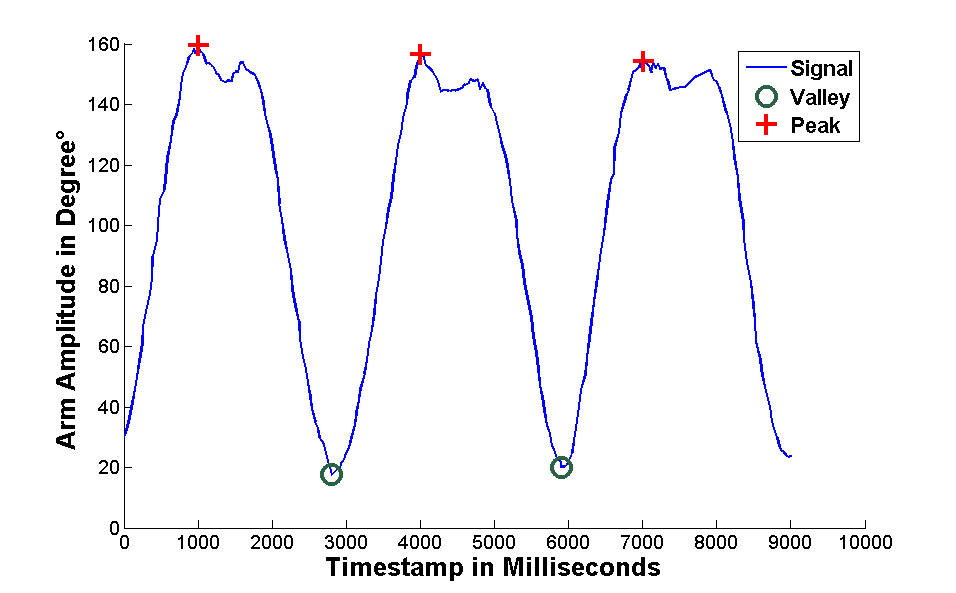
\includegraphics[width=0.5\textwidth]{img/signalamplitudepeakvaley-2.png}
	\caption{Example of the angle over time with the peak and valley detection technique.}
	\label{fig:signalamplitudepeakvaley}
\end{figure}

The next phase of this research is to classify the motion data to identify the occurrence of Bradykinesia symptom. Using the theory of statistical learning, we have performed a data analysis to acquire knowledge through supervised learning methods, as explained in Section~\ref{classifier_performance}.

\section{Experiments and discussion}
\label{sec:experimentalresults}

This research project was approved by the Brazilian Ethic Committee of Federal University of Campina Grande with CAAE: 14408213.9.1001.5182. The research subjects were instructed about the procedures and signed a written informed consent.
%The research subjects played the game (\emph{Catch the Spheres}) with a MS-Kinect (Version 1.0) motion sensor and the HMS acquired and classified the user's motor data.

\subsection{Research Subjects}

A total number of 30 subjects participated in the study. The group previously diagnosed by neurologists with PD consisted of 15 subjects, 10 men and 5 women, between 51 and 65 years (mean: 58). The control group was composed of 15 subjects without a PD diagnosis, 11 men and 4 women, between 50 and 65 years (mean: 57). All subjects were interacting with exactly the same system in both hardware and software, and were prompted to seamlessly perform abduction and adduction of the arms according to the game's context. All sessions were made in a medical institution under the supervision of a neurologist or physiotherapist to continuously check the subject's health condition. No subject needed to interrupt the experiment to ensure safety.

\subsection{Data Collection}

The data collection was performed over a period of 2 months, on different days, at the same location, with each subject individually. Due to time constraints and technical requirements, such as to capture with the motion sensor the entire length of the upper arm during abduction and adduction movements, each subject was instructed to perform the following steps:

\begin{compactenum}
	\item The subject stands at distance of 2 meters from the motion sensor at a place marked for that purpose on the ground.
	\item The subject faces a projection of the game on a wall, centered over the motion sensor.
	\item The subject plays the game \textit{Catch the Spheres} for 5 minutes.
	\item The subjects end the game by reaching the virtual exit button (seen as a button with an 'X' in Fig.~\ref{img:catch}).
\end{compactenum} 

\subsection{SVM Classifier Performance}
\label{classifier_performance}

The SVM is a supervised learning algorithm that creates learning functions from a set of labeled training data. We selected this approach because it requires a relatively small number of samples for training \cite{kantardzic2011data}. This algorithm has a good generalization to discriminate between two classes represented as $n$-dimensional vectors with a discriminant function resulting in a binary output.

In this work, we applied the grid search technique \cite{kantardzic2011data} to identify the best SVM parameters, using Leave-One-Out Cross-Validation (LOOCV). This technique assesses the accuracy of the predicted model, prevents the over fitting problem in the binary classification and is a practical method to identify the SVM parameters. In this study, to reduce the error rate, we applied a mini max approach to maximize the margin over the hyper plane coefficients and the correct classification.


The best classification performance of this study is presented in the confusion matrix \cite{kantardzic2011data} for two classes that consist of a matrix $2$\ x $2$\, with (TP, FP, TN and FN) described in Table~\ref{table:resultadomatrizconfusaosvm} and his metrics is presented in the Table~\ref{table:metricas}.

\begin{table}[!htbp]
\caption{Confusion Matrix Of SVM Classification With One Leave Out Cross Validation.}
\label{table:resultadomatrizconfusaosvm}
\centering
\begin{tabular}{l|c|c|}
\cline{2-3}
\multicolumn{1}{c}{}                         & \multicolumn{2}{|c|}{\textit{\textbf{Predicted Class}}} \\ \cline{2-3} 
                                             & \textbf{Parkinson}      & \textbf{Control Group}         \\ \hline
\multicolumn{1}{|l|}{\textbf{Parkinson}} & 12       & 3          \\ \hline
\multicolumn{1}{|l|}{\textbf{Control Group}}     & 1           & 14     \\ \hline
\end{tabular}
\end{table}


We assessed bradykinesia by measuring the amplitude and angular velocities in the adduction and abduction movements of the subjects. Therefore, the amplitude and angular velocities were the feature vectors for data classification~\cite{kantardzic2011data}. In Table~\ref{table:amplitude}, we show the severity of motor disorder caused by bradykinesia, in which PD's patients present lower amplitudes. Notice that subject Control 10 presents amplitude values similar to the PD's patients. In this case, we checked that this subject has an uninformed motor disorder that caused the incorrect classification. Furthermore, some PD's patients, namely Parkinson 3,8 and 12, did not present the bradykinesia symptom. In this case, we assumed that these subjects did not have the symptom or it was successfully suppressed by medication. 

\begin{table}[!h]
\centering
\caption{Results of Arm Abduction Amplitude}
\label{table:amplitude}
\begin{tabular}{|l|l|l|l|}
\hline
\rowcolor[HTML]{EFEFEF} 
\textbf{Subjects} & \textbf{\begin{tabular}[c]{@{}l@{}}Mean of\\ Amplitude \\ Left {[\degree]}\end{tabular}} & \textbf{\begin{tabular}[c]{@{}l@{}}Mean of\\ Amplitude\\ Right {[\degree]}\end{tabular}} & \textbf{\begin{tabular}[c]{@{}l@{}}Predicted\\ Class\end{tabular}} \\ \hline
Control 1         & \multicolumn{1}{r|}{153.62}                                                          & \multicolumn{1}{r|}{151.14}                                                          & Control                                                            \\ \hline
Control 2         & \multicolumn{1}{r|}{165.31}                                                          & \multicolumn{1}{r|}{151.84}                                                          & Control                                                            \\ \hline
Control 3         & \multicolumn{1}{r|}{155.44}                                                          & \multicolumn{1}{r|}{163.31}                                                          & Control                                                            \\ \hline
Control 4         & \multicolumn{1}{r|}{169.12}                                                          & \multicolumn{1}{r|}{169.39}                                                          & Control                                                            \\ \hline
Control 5         & \multicolumn{1}{r|}{157.20}                                                          & \multicolumn{1}{r|}{162.72}                                                          & Control                                                            \\ \hline
Control 6         & \multicolumn{1}{r|}{162.99}                                                          & \multicolumn{1}{r|}{167.25}                                                          & Control                                                            \\ \hline
Control 7         & \multicolumn{1}{r|}{166.90}                                                          & \multicolumn{1}{r|}{166.93}                                                          & Control                                                            \\ \hline
Control 8         & \multicolumn{1}{r|}{154.68}                                                          & \multicolumn{1}{r|}{159.13}                                                          & Control                                                            \\ \hline
Control 9         & \multicolumn{1}{r|}{162.31}                                                          & \multicolumn{1}{r|}{158.17}                                                          & Control                                                            \\ \hline
Control 10         & \multicolumn{1}{r|}{135.22}                                                          & \multicolumn{1}{r|}{131.85}                                                          & \textbf{Parkinson}                                                            \\ \hline
Control 11         & \multicolumn{1}{r|}{162.13}                                                          & \multicolumn{1}{r|}{167.61}                                                          & Control                                                            \\ \hline
Control 12         & \multicolumn{1}{r|}{161.69}                                                          & \multicolumn{1}{r|}{166.78}                                                          & Control                                                            \\ \hline
Control 13         & \multicolumn{1}{r|}{160.47}                                                          & \multicolumn{1}{r|}{155.05}                                                          & Control                                                            \\ \hline
Control 14         & \multicolumn{1}{r|}{174.37}                                                          & \multicolumn{1}{r|}{167.66}                                                          & Control                                                            \\ \hline
Control 15         & \multicolumn{1}{r|}{155.08}                                                          & \multicolumn{1}{r|}{167.83}                                                          & Control                                                            \\ \hline
Parkinson 1         & \multicolumn{1}{r|}{125.80}                                                          & \multicolumn{1}{r|}{119.73}                                                          & Parkinson                                                            \\ \hline
Parkinson 2         & \multicolumn{1}{r|}{131.28}                                                          & \multicolumn{1}{r|}{123.49}                                                          & Parkinson                                                            \\ \hline
Parkinson 3         & \multicolumn{1}{r|}{156.66}                                                          & \multicolumn{1}{r|}{149.46}                                                          & \textbf{Control}                                                            \\ \hline
Parkinson 4         & \multicolumn{1}{r|}{139.90}                                                          & \multicolumn{1}{r|}{142.83}                                                          & Parkinson                                                            \\ \hline
Parkinson 5         & \multicolumn{1}{r|}{147.37}                                                          & \multicolumn{1}{r|}{153.13}                                                          & Parkinson                                                            \\ \hline
Parkinson 6         & \multicolumn{1}{r|}{115.32}                                                          & \multicolumn{1}{r|}{123.56}                                                          & Parkinson                                                            \\ \hline
Parkinson 7         & \multicolumn{1}{r|}{129.75}                                                          & \multicolumn{1}{r|}{133.04}                                                          & Parkinson                                                            \\ \hline
Parkinson 8         & \multicolumn{1}{r|}{166.62}                                                          & \multicolumn{1}{r|}{165.63}                                                          & \textbf{Control}                                                            \\ \hline
Parkinson 9         & \multicolumn{1}{r|}{143.95}                                                          & \multicolumn{1}{r|}{140.45}                                                          & Parkinson                                                            \\ \hline
Parkinson 10         & \multicolumn{1}{r|}{136.86}                                                          & \multicolumn{1}{r|}{151.03}                                                          & Parkinson                                                            \\ \hline
Parkinson 11         & \multicolumn{1}{r|}{156.87}                                                          & \multicolumn{1}{r|}{142.93}                                                          & Parkinson                                                            \\ \hline
Parkinson 12         & \multicolumn{1}{r|}{166.59}                                                          & \multicolumn{1}{r|}{157.81}                                                          & \textbf{Control}                                                            \\ \hline
Parkinson 13         & \multicolumn{1}{r|}{147.99}                                                          & \multicolumn{1}{r|}{142.02}                                                          & Parkinson                                                            \\ \hline
Parkinson 14         & \multicolumn{1}{r|}{141.95}                                                          & \multicolumn{1}{r|}{150.60}                                                          & Parkinson                                                            \\ \hline
Parkinson 15         & \multicolumn{1}{r|}{125.69}                                                          & \multicolumn{1}{r|}{140.62}                                                          & Parkinson                                                            
\\ \hline
\end{tabular}
\end{table}

\begin{table}[htbp!]
\caption{Performance of PD and Control Group classification.}
\label{table:metricas}
\centering
\begin{tabular}{|l|r|}
\hline
\multicolumn{2}{|l|}{\textbf{Classifier Metrics}} \\ \hline
\textbf{TpRate}                    & 80.00$\%$\                 \\ \hline
\textbf{FpRate}                    & 6.67$\%$\                \\ \hline
\textbf{Accuracy}                  & 86.67$\%$\                \\ \hline
\textbf{F-score}                   & 85.71$\%$\                \\ \hline
\textbf{Precision}                  & 92.31$\%$\                \\ \hline
\end{tabular}
\end{table}

\subsection{User Acceptance with the GQM Results}

Goal Question Metric (GQM) \cite{gqmhci2009} is a goal-oriented paradigm to define measurements based on explicit and precisely defined goals.  Based on the GQM paradigm, we defined two goals following the GQM template presented in \cite{gqmhci2009}: 

%GQM has a hierarchical structure divided into three levels: \texttt{Goal}, the conceptual level defined for an object of measurement, such as products, processes and resources; \texttt{Question}, the operational level in which a set of questions is used to decide if a specific goal was achieved; and \texttt{Metric}, the quantitative level in which a set of data is collected to answer the questions from the \texttt{Question} level in a quantitative way.

\begin{compactitem}
	\item G1: Analyze our HMS PD approach for the purpose of evaluating with respect to usability from the view point of the patients in the context of the game \emph{Catch the Spheres}
	\item G2: Analyze our HMS PD approach for the purpose of evaluating with respect to fit to daily routine from the view point of the patients in the context of the game \emph{Catch the Spheres}
\end{compactitem}

For G1 we defined two questions: 

\begin{compactitem}
	\item Q1: Is the game a good entertainment and do PD patients feel motivated to play it again?
	\item Q2: Is the game simple, without many rules, and understandable? Could it be played by PD patients of different ages? 
\end{compactitem}

For G2 we defined three questions:

\begin{compactitem}
	\item Q3: Are PD patients used to playing casual games at home?
	\item Q4: Could PD patients integrate this game into their daily routine?
	\item Q5: Would an elderly user be safe in playing this game using the arms movements?
\end{compactitem}

For each question, we defined a measurement to be collected using a Boolean scale (i.e., \emph{yes} and \emph{no}). The measurements were collected through a questionnaire and we obtained the following result indicating that we reached our goals: 90\% of the users felt motivated with the game (Q1); 93\% found the game simple and could be played by people of different ages (Q2); only 53\% of the respondents are used to play casual games at home (Q3); 80\% would add this game-based monitoring approach into their daily routine (Q4); 75\% considered it safe for elderly users (Q5).

\section{Conclusion}
\label{conclusion}

In this work we presented a game-based approach to monitor the motor symptoms of Parkinson's Disease. The game was applied to motivate the user to be monitored, allowing the collection of biomechanical data measurements. We monitored PD symptoms through the abduction and adduction arm movements, calculating the amplitude and its respective angular velocity to assess bradykinesia motor symptom. This method is commonly applied by neurologists at consultation to distinguish normal and abnormal movements. In this way, we enable the monitoring of PD patients at home, increasing the frequency of symptoms measurement.

To evaluate our approach, we performed an experimental study with 30 research subjects divided in PD and Control group. We used SVM to identify the occurrence of PD's bradykinesia motor symptom and had a classification \textit{Precision} of 92.31\%. Moreover, 90,00\% of the patients considered our approach non-invasive and easy to integrate into their routine. 

%For future works, we plan to further identify the variance of the PD's bradykinesia during a medication cycle.

%For future works, we plan to further identify PD symptoms such as dyskinesia and tremor and evaluate our approach with PD patients in different scenarios. Thus, we intend to identify the variance of the PD's motor symptoms during a medication cycle to improve the quality of the information available to the health professional.


\bibliographystyle{IEEEtran}
\bibliography{sigproc2,IEEEFormat}

\end{document}